\setcounter{section}{19}
\setcounter{subsection}{10}
\setcounter{subsubsection}{3}
% Copyright 2019 by Till Tantau
%
% This file may be distributed and/or modified
%
% 1. under the LaTeX Project Public License and/or
% 2. under the GNU Free Documentation License.
%
% See the file doc/generic/pgf/licenses/LICENSE for more details.


\section{Matrices and Alignment\\矩阵和对齐}
\label{section-matrices}

\subsection{Overview\\概述}

When creating pictures, one often faces the problem of correctly aligning parts
of the picture. For example, you might wish that the |baseline|s of certain
nodes should be on the same line and some further nodes should be below these
nodes with, say, their centers on a vertical lines. There are different ways of
solving such problems. For example, by making clever use of anchors, nearly all
such alignment problems can be solved. However, this often leads to complicated
code. An often simpler way is to use \emph{matrices}, the use of which is
explained in the current section.

在创建图片时,通常面临正确对齐图片部分的问题。例如,您可能希望某些节点的 |baseline| 在同一行上,而一些其他节点应该位于这些节点的下方,例如,它们的中心在垂直线上。解决这类问题有不同的方法。例如,通过巧妙地使用锚点,几乎可以解决所有这些对齐问题。然而,这通常会导致复杂的代码。一个通常更简单的方法是使用\emph{矩阵},本节将介绍矩阵的使用方法。

A \tikzname\ matrix is similar to \LaTeX's |{tabular}| or |{array}|
environment, only instead of text each cell contains a little picture or a
node. The sizes of the cells are automatically adjusted such that they are
large enough to contain all the cell contents.

\tikzname\ 矩阵类似于 \LaTeX\ 的 |{tabular}| 或 |{array}| 环境,只是每个单元格中包含的是一个小图片或一个节点,单元格的大小会自动调整,使其足够大以容纳所有单元格内容。

Matrices are a powerful tool and they need to be handled with some care. For
impatient readers who skip the rest of this section: you \emph{must} end
\emph{every} row with |\\|. In particular, the last row \emph{must} be ended
with |\\|.

矩阵是一个强大的工具,需要谨慎使用。对于急躁的读者,如果跳过本节的其余内容:您\emph{必须}在\emph{每一行}的末尾使用 |\\|。特别是,最后一行\emph{必须}以 |\\| 结束。

Many of the ideas implemented in \tikzname's matrix support are due to Mark
Wibrow -- many thanks to Mark at this point!

许多在 \tikzname\ 的矩阵支持中实现的想法归功于 Mark Wibrow - 在此向 Mark 表示感谢!
\subsection{Matrices are Nodes\\矩阵是节点}

Matrices are special in many ways, but for most purposes matrices are treated
like nodes. This means, that you use the |node| path command to create a matrix
and you only use a special option, namely the |matrix| option, to signal that
the node will contain a matrix. Instead of the usual \TeX-box that makes up the
|text| part of the node's shape, the matrix is used. Thus, in particular, a
matrix can have a shape, this shape can be drawn or filled, it can be used in a
tree, and so on. Also, you can refer to the different anchors of a matrix.

矩阵在许多方面都是特殊的,但对于大多数目的,矩阵被视为节点。这意味着您可以使用 |node| 路径命令创建一个矩阵,并且只需要使用一个特殊选项,即 |matrix| 选项,来表示节点将包含一个矩阵。矩阵使用的是整个 \TeX 盒子,而不是节点形状的 |text| 部分。因此,特别地,矩阵可以具有形状,可以绘制或填充该形状,可以在树中使用,等等。此外,您还可以引用矩阵的不同锚点。

\begin{key}{/tikz/matrix=\meta{true or false} (default true)}
    This option can be passed to a |node| path command. It signals that the
    node will contain a matrix.

    此选项可以传递给 |node| 路径命令。它表示节点将包含一个矩阵。
    %
\begin{codeexample}[]
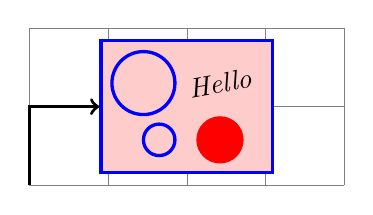
\begin{tikzpicture}
  \draw[help lines] (0,0) grid (4,2);
  \node [matrix,fill=red!20,draw=blue,very thick] (my matrix) at (2,1)
  {
    \draw (0,0)   circle (4mm); & \node[rotate=10] {Hello};        \\
    \draw (0.2,0) circle (2mm); & \fill[red]   (0,0) circle (3mm); \\
  };

  \draw [very thick,->] (0,0) |- (my matrix.west);
\end{tikzpicture}
\end{codeexample}
    %
    The exact syntax of the matrix is explained in the course of this section.
    
    矩阵的确切语法将在本节中讲解。


    \begin{stylekey}{/tikz/every matrix (initially \normalfont empty)}
        This style is used in every matrix.

        此样式在每个矩阵中使用。

    \end{stylekey}
    %
    \begin{stylekey}{/tikz/every outer matrix (initially \normalfont empty)}
        While the |every matrix| key also applies to the matrix contents, this
        only applies to the outer node which holds the matrix.
    
        尽管 |every matrix| 键也适用于矩阵内容,但这仅适用于包含矩阵的外部节点。

      \end{stylekey}
\end{key}

Even more so than nodes, matrices will often be the only object on a path.
Because of this, there is a special abbreviation for creating matrices:

与节点不同,矩阵通常是路径上唯一的对象。因此,有一个特殊的缩写方式来创建矩阵:

\begin{command}{\matrix}
    Inside |{tikzpicture}| this is an abbreviation for |\path node[matrix]|.

    在 |{tikzpicture}| 中,这是 |\path node[matrix]| 的缩写。
  \end{command}

Even though matrices are nodes, some options do not have the same effect as for
normal nodes:

尽管矩阵是节点,但某些选项并没有像普通节点那样产生相同的效果:

%
\begin{enumerate}
    \item Rotations and scaling have no effect on a matrix as a whole (however,
        you can still transform the contents of the cells normally). Before the
        matrix is typeset, the rotational and scaling part of the
        transformation matrix is reset.

        旋转和缩放对整个矩阵没有影响(但是,您仍然可以正常地转换单元格的内容)。在矩阵排版之前,将重置变换矩阵的旋转和缩放部分。


    \item For multi-part shapes you can only set the |text| part of the node.

    对于多部分形状,您只能设置节点的 |text| 部分。


    \item All options starting with |text| such as |text width| have no effect.

    以 |text| 开头的所有选项,如 |text width|,没有效果。


    \item If you place a matrix on a path, the matrix contents will be
        collected into a macro, which tokenizes them.  This means that |&| will
        lose its meaning as an alignment character, resulting in an error.  If
        you need to place a matrix on a path, use |ampersand replacement| to
        work around that problem.

        如果将矩阵放置在路径上,则矩阵内容将被收集到一个宏中,并以令牌形式表示。这意味着 |&| 将失去其作为对齐字符的含义,导致错误。如果需要在路径上放置矩阵,请使用 |ampersand replacement| 来解决这个问题。


\end{enumerate}


\subsection{Cell Pictures\\单元格图片}
\label{section-tikz-cell-pictures}

A matrix consists of rows of \emph{cells}. Each row (including the last one!)
is ended by the command |\\|. The character |&| is used to separate cells.
Inside each cell, you must place commands for drawing a picture, called the
\emph{cell picture} in the following. (However, cell pictures are not enclosed
in a complete |{pgfpicture}| environment, they are a bit more light-weight. The
main difference is that cell pictures cannot have layers.) It is not necessary
to specify beforehand how many rows or columns there are going to be and if a
row contains less cell pictures than another line, empty cells are
automatically added as needed.

矩阵由一行一行的\emph{单元格}组成。每行(包括最后一行!)以命令 |\\| 结束。字符 |&| 用于分隔单元格。在每个单元格内,您必须放置绘制图片的命令,称为以下\emph{单元格图片}(cell picture)。(但是,单元格图片不包含在完整的 |{pgfpicture}| 环境中,它们更加轻量级。主要区别是单元格图片不能有层。)不需要预先指定将有多少行或列,如果一行的单元格图片少于另一行,将自动添加所需的空单元格。

\subsubsection{Alignment of Cell Pictures\\单元格图片的对齐}

For each cell picture a bounding box is computed. These bounding boxes and the
origins of the cell pictures determine how the cells are aligned. Let us start
with the rows: Consider the cell pictures on the first row. Each has a bounding
box and somewhere inside this bounding box the origin of the cell picture can
be found (the origin might even lie outside the bounding box, but let us ignore
this problem for the moment). The cell pictures are then shifted around such
that all origins lie on the same horizontal line. This may make it necessary to
shift some cell pictures upwards and others downwards, but it can be done and
this yields the vertical alignment of the cell pictures this row. The top of
the row is then given by the top of the ``highest'' cell picture in the row,
the bottom of the row is given by the bottom of the lowest cell picture. (To be
more precise, the height of the row is the maximum $y$-value of any of the
bounding boxes and the depth of the row is the negated minimum $y$-value of the
bounding boxes).

为每个单元格图片计算一个边界框。这些边界框和单元格图片的原点确定了单元格的对齐方式。让我们从行开始:考虑第一行的单元格图片。每个单元格图片都有一个边界框,而在边界框内的某个位置可以找到单元格图片的原点(原点甚至可能位于边界框之外,但我们暂时忽略这个问题)。然后,将单元格图片进行平移,使得所有原点位于同一条水平线上。这可能需要将一些单元格图片向上移动,将另一些单元格图片向下移动,但可以做到,从而得到了该行单元格图片的垂直对齐。行的顶部由该行中“最高”的单元格图片的顶部给出,行的底部由最低单元格图片的底部给出。(更准确地说,行的高度是任何边界框的最大 $y$ 值,行的深度是边界框的最小 $y$ 值的相反数)。

%
\begin{codeexample}[]
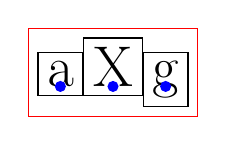
\begin{tikzpicture}
  [every node/.style={draw=black,anchor=base,font=\huge}]

  \matrix [draw=red]
  {
    \node {a}; \fill[blue] (0,0) circle (2pt); &
    \node {X}; \fill[blue] (0,0) circle (2pt); &
    \node {g}; \fill[blue] (0,0) circle (2pt); \\
  };
\end{tikzpicture}
\end{codeexample}

Each row is aligned in this fashion: For each row the cell pictures
are vertically aligned such that the origins lie on the same
line. Then the second row is placed below the first row such that the
bottom of the first row touches the top of the second row (unless a
|row sep| is used to add a bit of space). Then the bottom of the
second row touches the top of the third row, and so on. Typically,
each row will have an individual height and depth.

每一行都以这种方式对齐:对于每一行,单元格图片垂直对齐,使得它们的原点位于同一条线上。然后,第二行放置在第一行的下方,使得第一行的底部与第二行的顶部接触(除非使用 |row sep| 来添加一些空间)。然后,第二行的底部与第三行的顶部接触,依此类推。通常,每一行都会有独立的高度和深度。
\begin{codeexample}[]
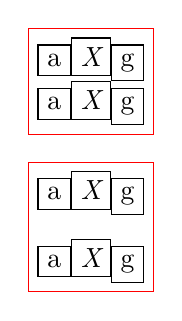
\begin{tikzpicture}
  [every node/.style={draw=black,anchor=base}]

  \matrix [draw=red]
  {
    \node {a}; & \node {X}; & \node {g}; \\
    \node {a}; & \node {X}; & \node {g}; \\
  };

  \matrix [row sep=3mm,draw=red] at (0,-2)
  {
    \node {a}; & \node {X}; & \node {g}; \\
    \node {a}; & \node {X}; & \node {g}; \\
  };
\end{tikzpicture}
\end{codeexample}

Let us now have a look at the columns. The rules for how the pictures on any
given column are aligned are very similar to the row alignment: Consider all
cell pictures in the first column. Each is shifted horizontally such that the
origins lie on the same vertical line. Then, the left end of the column is at
the left end of the bounding box that protrudes furthest to the left. The right
end of the column is at the right end of the bounding box that protrudes
furthest to the right. This fixes the horizontal alignment of the cell pictures
in the first column and the same happens the cell pictures in the other
columns. Then, the right end of the first column touches the left end of the
second column (unless |column sep| is used). The right end of the second column
touches the left end of the third column, and so on. (Internally, two columns
are actually used to achieve the desired horizontal alignment, but that is only
an implementation detail.)

现在让我们来看看列。列上的图片的对齐规则与行的对齐非常相似:考虑第一列中的所有单元格图片。每个单元格图片都会水平平移,使得原点位于同一条垂直线上。然后,该列的左端位于最左边的边界框的左端。该列的右端位于最右边的边界框的右端。这确定了第一列中单元格图片的水平对齐方式,并且决定了其他列中的单元格图片的对齐方式。然后,第一列的右端与第二列的左端接触(除非使用 |column sep|)。第二列的右端与第三列的左端接触,依此类推。(在内部,实际上使用了两列来实现所需的水平对齐,但这只是一个实现细节)。


\begin{codeexample}[]
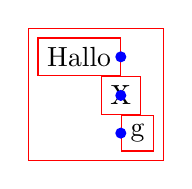
\begin{tikzpicture}[every node/.style={draw}]
  \matrix [draw=red]
  {
    \node[left]  {Hallo}; \fill[blue] (0,0) circle (2pt); \\
    \node        {X};     \fill[blue] (0,0) circle (2pt); \\
    \node[right] {g};     \fill[blue] (0,0) circle (2pt); \\
  };
\end{tikzpicture}
\end{codeexample}

\begin{codeexample}[]
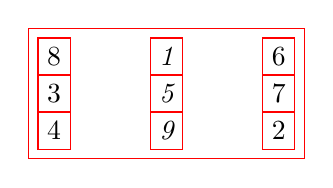
\begin{tikzpicture}[every node/.style={draw}]
  \matrix [draw=red,column sep=1cm]
  {
    \node {8}; & \node{1}; & \node {6}; \\
    \node {3}; & \node{5}; & \node {7}; \\
    \node {4}; & \node{9}; & \node {2}; \\
  };
\end{tikzpicture}
\end{codeexample}


\subsubsection{Setting and Adjusting Column and Row Spacing\\设置和调整列和行间距}

There are different ways of setting and adjusting the spacing between columns
and rows. First, you can use the options |column sep| and |row sep| to set a
default spacing for all rows and all columns. Second, you can add options to
the |&| character and the |\\| command to adjust the spacing between two
specific columns or rows. Additionally, you can specify whether the space
between two columns or rows should be considered between the origins of cells
in the column or row or between their borders.

有不同的方法可以设置和调整列和行之间的间距。首先,可以使用选项 |column sep| 和 |row sep| 来为所有行和列设置默认间距。其次,可以在 |&| 字符和 |\\| 命令上添加选项,以调整两个特定列或行之间的间距。此外,还可以指定两个列或行之间的空间是在单元格的原点之间还是在边界之间。

\begin{key}{/tikz/column sep=\meta{spacing list}}
    This option sets a default space that is added between every two columns.
    This space can be positive or negative and is zero by default. The
    \meta{spacing list} normally contains a single dimension like |2pt|.

    该选项设置在每两列之间添加的默认间距。该间距可以是正数或负数,默认为零。\meta{spacing list} 通常包含一个单独的尺寸,如 |2pt|。
    %
\begin{codeexample}[]
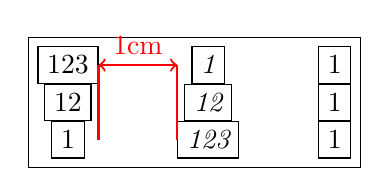
\begin{tikzpicture}
  \matrix [draw,column sep=1cm,nodes=draw]
  {
    \node(a) {123}; & \node (b) {1};   & \node {1}; \\
    \node    {12};  & \node     {12};  & \node {1}; \\
    \node(c) {1};   & \node (d) {123}; & \node {1}; \\
  };
  \draw [red,thick]  (a.east) -- (a.east |- c)
                     (d.west) -- (d.west |- b);
  \draw [<->,red,thick] (a.east) -- (d.west |- b)
    node [above,midway] {1cm};
\end{tikzpicture}
\end{codeexample}
    %
    More generally, the \meta{spacing list} may contain a whole list of
    numbers, separated by commas, and occurrences of the two key words
    |between origins| and |between borders|. The effect of specifying such a
    list is the following: First, all numbers occurring in the list are simply
    added to compute the final spacing. Second, concerning the two keywords,
    the last occurrence of one of the keywords is important. If the last
    occurrence is |between borders| or if neither occurs, then the space is
    inserted between the two columns normally. However, if the last occurs is
    |between origins|, then the following happens: The distance between the
    columns is adjusted such that the difference between the origins of all the
    cells in the first column (remember that they all lie on straight line) and
    the origins of all the cells in the second column is exactly the given
    distance.

    更一般地,\meta{spacing list} 可以包含一个由逗号分隔的整个数字列表,以及关键字 |between origins| 和 |between borders| 的出现次数。指定这样一个列表的效果如下:首先,列表中出现的所有数字都会简单相加以计算最终的间距。其次,在关键字方面,最后出现的关键字很重要。如果最后出现的是 |between borders|,或者两者都没有出现,则空间通常插入在两个列之间。然而,如果最后出现的是 |between origins|,则会发生以下情况:调整列之间的距离,使得第一列中所有单元格的原点(记住它们都位于一条直线上)与第二列中所有单元格的原点之间的差正好等于给定的距离。

    \emph{The }|between origins|\emph{ option can only be used for columns
    mentioned in the first row, that is, you cannot specify this option for
    columns introduced only in later rows.}

    \emph{|between origins| 选项只能用于第一行中提到的列,也就是说,不能为仅在后续行中引入的列指定此选项。}

    %
\begin{codeexample}[]
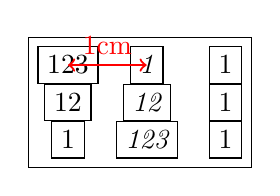
\begin{tikzpicture}
  \matrix [draw,column sep={1cm,between origins},nodes=draw]
  {
    \node(a) {123}; & \node (b) {1};   & \node {1}; \\
    \node    {12};  & \node     {12};  & \node {1}; \\
    \node    {1};   & \node     {123}; & \node {1}; \\
  };
  \draw [<->,red,thick] (a.center) -- (b.center) node [above,midway] {1cm};
\end{tikzpicture}
\end{codeexample}
    %
\end{key}

\begin{key}{/tikz/row sep=\meta{spacing list}}
    This option works like |column sep|, only for rows. Here, too, you can
    specify whether the space is added between the lower end of the first row
    and the upper end of the second row, or whether the space is computed
    between the origins of the two rows.
    
    该选项与 |column sep| 类似,只是针对行。在这里,您也可以指定空间是在第一行的下端和第二行的上端之间添加,还是计算两行的原点之间的空间。

%
\begin{codeexample}[]
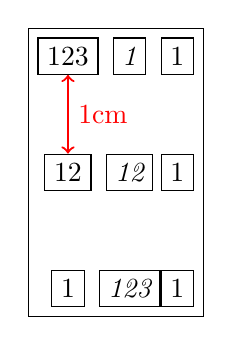
\begin{tikzpicture}
  \matrix [draw,row sep=1cm,nodes=draw]
  {
    \node (a) {123}; & \node {1};   & \node {1}; \\
    \node (b) {12};  & \node {12};  & \node {1}; \\
    \node     {1};   & \node {123}; & \node {1}; \\
  };
  \draw [<->,red,thick] (a.south) -- (b.north) node [right,midway] {1cm};
\end{tikzpicture}
\end{codeexample}
    %
\begin{codeexample}[]
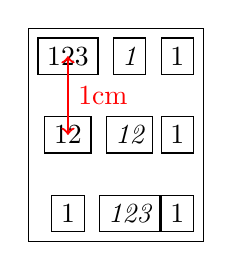
\begin{tikzpicture}
  \matrix [draw,row sep={1cm,between origins},nodes=draw]
  {
    \node (a) {123}; & \node {1};   & \node {1}; \\
    \node (b) {12};  & \node {12};  & \node {1}; \\
    \node     {1};   & \node {123}; & \node {1}; \\
  };
  \draw [<->,red,thick] (a.center) -- (b.center) node [right,midway] {1cm};
\end{tikzpicture}
\end{codeexample}
    %
\end{key}

The row-end command |\\| allows you to provide an optional argument, which must
be a dimension. This dimension will be added to the list in |row sep|. This
means that, firstly, any numbers you list in this argument will be added as an
extra row separation between the line being ended and the next line and,
secondly, you can use the keywords |between origins| and |between borders| to
locally overrule the standard setting for this line pair.
%

行结束命令 |\\| 允许您提供一个可选参数,该参数必须是一个尺寸。该尺寸将添加到 |row sep| 中的列表中。这意味着,首先,您在此参数中列出的任何数字都将作为额外的行间隔添加到结束的行和下一行之间,其次,您可以使用关键字 |between origins| 和 |between borders| 在本地覆盖此行对的标准设置。

\begin{codeexample}[]
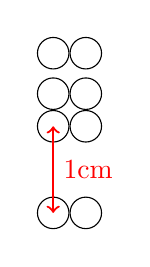
\begin{tikzpicture}
  \matrix [row sep=1mm]
  {
    \draw (0,0) circle (2mm); & \draw (0,0) circle (2mm); \\
    \draw (0,0) circle (2mm); & \draw (0,0) circle (2mm); \\[-1mm]
    \draw (0,0) coordinate (a) circle (2mm); &
    \draw (0,0) circle (2mm); \\[1cm,between origins]
    \draw (0,0) coordinate (b) circle (2mm); &
    \draw (0,0) circle (2mm); \\
  };
  \draw [<->,red,thick] (a.center) -- (b.center) node [right,midway] {1cm};
\end{tikzpicture}
\end{codeexample}

The cell separation character |&| also takes an optional argument, which must
also be a spacing list. This spacing list is added to the |column sep| having a
similar effect as the option for the |\\| command for rows.

单元格分隔符 |&| 也可以带有一个可选参数,该参数也必须是一个间距列表。此间距列表会添加到 |column sep| 中,类似于行的 |\\| 命令的选项对行的影响。

This optional spacing list can only be given the first time a new column is
started (usually in the first row), subsequent usages of this option in later
rows have no effect.

此可选间距列表只能在开始新列时给出(通常在第一行中),在后续行中对该选项的重复使用没有影响。

%
\begin{codeexample}[]
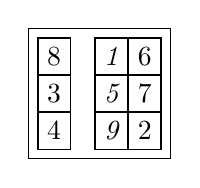
\begin{tikzpicture}
  \matrix [draw,nodes=draw,column sep=1mm]
  {
    \node {8}; &[2mm] \node{1}; &[-1mm] \node {6}; \\
    \node {3}; &      \node{5}; &       \node {7}; \\
    \node {4}; &      \node{9}; &       \node {2}; \\
  };
\end{tikzpicture}
\end{codeexample}
%
\begin{codeexample}[]
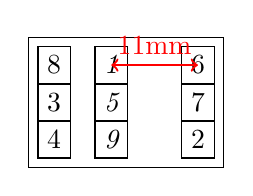
\begin{tikzpicture}
  \matrix [draw,nodes=draw,column sep=1mm]
  {
    \node {8}; &[2mm] \node(a){1}; &[1cm,between origins] \node(b){6}; \\
    \node {3}; &      \node   {5}; &                      \node   {7}; \\
    \node {4}; &      \node   {9}; &                      \node   {2}; \\
  };
  \draw [<->,red,thick] (a.center) -- (b.center) node [above,midway] {11mm};
\end{tikzpicture}
\end{codeexample}
%
\begin{codeexample}[]
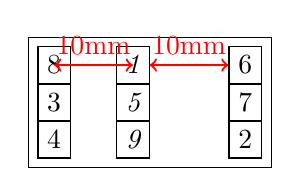
\begin{tikzpicture}
  \matrix [draw,nodes=draw,column sep={1cm,between origins}]
  {
    \node (a) {8}; & \node (b) {1}; &[between borders] \node (c) {6}; \\
    \node     {3}; & \node     {5}; &                  \node     {7}; \\
    \node     {4}; & \node     {9}; &                  \node     {2}; \\
  };
  \draw [<->,red,thick] (a.center) -- (b.center) node [above,midway] {10mm};
  \draw [<->,red,thick] (b.east) -- (c.west) node [above,midway] {10mm};
\end{tikzpicture}
\end{codeexample}


\subsubsection{Cell Styles and Options\\单元格样式和选项}

The following styles and options are useful for changing the appearance of all
cell pictures:

以下样式和选项对于更改所有单元格图片的外观非常有用:

\begin{stylekey}{/tikz/every cell=\marg{row}\marg{column} (initially \normalfont empty)}
    This style is installed at the beginning of each cell picture with the two
    parameters being the current \meta{row} and \meta{column} of the cell. Note
    that setting this style to |draw| will \emph{not} cause all nodes to be
    drawn since the |draw| option has to be passed to each node individually.

    此样式安装在每个单元格图片的开头,两个参数是单元格的当前\meta{row}和\meta{column}。请注意,将此样式设置为|draw|不会导致所有节点都被绘制,因为|draw|选项必须分别传递给每个节点。

    Inside this style (and inside all cells), the current \meta{row} and
    \meta{column} number are also accessible via the counters
    |\pgfmatrixcurrentrow| and |\pgfmatrixcurrentcolumn|.

    在此样式(以及所有单元格)内部,当前的\meta{row}和\meta{column}编号也可以通过计数器|\pgfmatrixcurrentrow|和|\pgfmatrixcurrentcolumn|访问。

  \end{stylekey}

\begin{key}{/tikz/cells=\meta{options}}
    This key adds the \meta{options} to the style |every cell|. It is mainly
    just a shorthand for the code |every cell/.append style=|\meta{options}.

    此键将\meta{options}添加到样式|every cell|。它主要只是代码|every cell/.append style=|\meta{options}的简写形式。

  \end{key}

\begin{key}{/tikz/nodes=\meta{options}}
    This key adds the \meta{options} to the style |every node|. It is mainly
    just a shorthand for the code |every node/.append style=|\meta{options}.

    此键将\meta{options}添加到样式|every node|。它主要只是代码|every node/.append style=|\meta{options}的简写形式。

    The main use of this option is the install some options for the nodes
    \emph{inside} the matrix that should not apply to the matrix \emph{itself}.

    此选项的主要用途是为矩阵内部的节点安装一些不适用于矩阵本身的选项。

    %
\begin{codeexample}[]
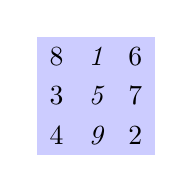
\begin{tikzpicture}
  \matrix [nodes={fill=blue!20,minimum size=5mm}]
  {
    \node {8}; & \node{1}; & \node {6}; \\
    \node {3}; & \node{5}; & \node {7}; \\
    \node {4}; & \node{9}; & \node {2}; \\
  };
\end{tikzpicture}
\end{codeexample}
    %
\end{key}

The next set of styles can be used to change the appearance of certain rows,
columns, or cells. If more than one of these styles is defined, they are
executed in the below order (the |every cell| style is executed before all of
the below).

下一组样式可用于更改特定行、列或单元格的外观。如果定义了多个这些样式,则按照以下顺序执行(在下面的样式之前执行|every cell|样式)。

%
\begin{stylekey}{/tikz/column \meta{number}}
    This style is used for every cell in column \meta{number}.

    此样式用于第\meta{number}列的每个单元格。

  \end{stylekey}

\begin{stylekey}{/tikz/every odd column}
    This style is used for every cell in an odd column.

    此样式用于奇数列的每个单元格。

  \end{stylekey}

\begin{stylekey}{/tikz/every even column}
    This style is used for every cell in an even column.

    此样式用于偶数列的每个单元格。

  \end{stylekey}

\begin{stylekey}{/tikz/row \meta{number}}
    This style is used for every cell in row \meta{number}.

    此样式用于第\meta{number}行的每个单元格。

  \end{stylekey}

\begin{stylekey}{/tikz/every odd row}
    This style is used for every cell in an odd row.

    此样式用于奇数行的每个单元格。

  \end{stylekey}

\begin{stylekey}{/tikz/every even row}
    This style is used for every cell in an even row.

    此样式用于偶数行的每个单元格。

  \end{stylekey}

\begin{stylekey}{/tikz/row \meta{row number} column \meta{column number}}
    This style is used for the cell in row \meta{row number} and column
    \meta{column number}.

    此样式用于位于第\meta{row number}行和\meta{column number}列的单元格。

  \end{stylekey}
%
\begin{codeexample}[]
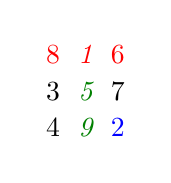
\begin{tikzpicture}
  [row 1/.style={red},
   column 2/.style={green!50!black},
   row 3 column 3/.style={blue}]

  \matrix
  {
    \node {8}; & \node{1}; & \node {6}; \\
    \node {3}; & \node{5}; & \node {7}; \\
    \node {4}; & \node{9}; & \node {2}; \\
  };
\end{tikzpicture}
\end{codeexample}

You can use the |column |\meta{number} option to change the alignment for
different columns.

您可以使用|column |\meta{number}选项来更改不同列的对齐方式。

%
\begin{codeexample}[]
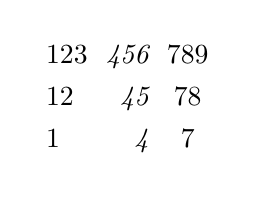
\begin{tikzpicture}
  [column 1/.style={anchor=base west},
   column 2/.style={anchor=base east},
   column 3/.style={anchor=base}]
  \matrix
  {
    \node {123}; & \node{456}; & \node {789}; \\
    \node {12}; & \node{45}; & \node {78}; \\
    \node {1}; & \node{4}; & \node {7}; \\
  };
\end{tikzpicture}
\end{codeexample}

In some cases, it is desirable to include some automation in each column/row
separately. A typical example is to apply stripe-pattern to almost all columns
with exceptions. For these type of use-cases, nesting these keys can open up
a lot of possibilities; in the following example a ``feature comparison'' table
is demonstrated. It is intentionally made rather verbose and a bit redundant
to show how the column and row settings can be progressively overwritten to
create certain effects.

在某些情况下,希望对每个列/行单独包含一些自动化。一个典型的示例是对几乎所有列应用条纹模式,但有例外情况。对于这类用例,嵌套这些键可以打开很多可能性;在下面的示例中,演示了一个“功能比较”表。它故意显得相当冗长和有些冗余,以显示可以逐步覆盖列和行设置以创建特定效果。

\begin{codeexample}[preamble={\usetikzlibrary{matrix,fit}}]
\begin{tikzpicture}[
  font=\sffamily,
  striped col/.style={column #1/.append style={
        every even row/.style={nodes={fill=olive!50}}}},
  head color/.style args={#1/#2}{column #1/.append style={
        row 1/.append style={nodes={fill=#2}}}}
]

\matrix [
   matrix of nodes, nodes in empty cells,
   nodes={text width=2cm, align=center,
          minimum height=1.5em, anchor=center},
   striped col/.list={1,...,5}, % add striped col style to all cols
   column 1/.style={ % Override stripes and modify the feature column
     row 1 column 1/.style={nodes={fill=none, draw=none}},
     nodes={fill=olive, inner ysep=0},
   },
   % modify headers first via common styles and then specific colors
   row 1/.style={nodes={text depth=0.2ex, text width=2cm, text=white}},
   head color/.list={2/orange,3/teal,4/cyan,5/magenta}
  ] (m)
  {
            & Basic     & Standard   & Professional & Enterprise \\
  Feature A & $\bullet$ & $\bullet$  & $\bullet$    & $\bullet$  \\
  Feature B & $\bullet$ & $\bullet$  & $\bullet$    & $\bullet$  \\
  Feature C &           &            &              & $\bullet$  \\
  Feature D &           & $\bullet$  & $\bullet$    & $\bullet$  \\
  Feature E &           &            & $\bullet$    & $\bullet$  \\
  };
% Add emphasis on selection by the use of "fit" library
\node[fit={(m-1-4.north west) (m-6-4.south east)},
      ultra thick, inner sep=0, rounded corners=1mm,
      draw=cyan, label={[cyan,align=center]270:Popular\\Choice!}]{};
\end{tikzpicture}
\end{codeexample}

The order in which these styles are applied is configurable.  You can also
install your own styles.  The following styles (in fact, internally they are
|/.code| keys) wrap the styles introduced in the previous paragraph passing the
correct argument and ensuring that they are only called for even or odd rows.
However, it is not recommended to override these.

应用这些样式的顺序是可配置的。您还可以安装自己的样式。以下样式(实际上,在内部它们是|/.code|键)包装了前面一段中引入的样式,传递正确的参数并确保仅对偶数或奇数行调用它们。但不建议覆盖这些样式。

\begin{stylekey}{/tikz/matrix/inner style/every cell}
    Wraps |/tikz/every cell|.
\end{stylekey}
\begin{stylekey}{/tikz/matrix/inner style/column}
    Wraps |/tikz/column |\meta{number}.
\end{stylekey}
\begin{stylekey}{/tikz/matrix/inner style/even odd column}
    Wraps |/tikz/every even column| and |/tikz/every odd column|.
\end{stylekey}
\begin{stylekey}{/tikz/matrix/inner style/row}
    Wraps |/tikz/row |\meta{number}.
\end{stylekey}
\begin{stylekey}{/tikz/matrix/inner style/even odd row}
    Wraps |/tikz/every even row| and |/tikz/every odd row|.
\end{stylekey}
\begin{stylekey}{/tikz/matrix/inner style/cell}
    Wraps |/tikz/row |\meta{number}| column |\meta{number}.
\end{stylekey}

\begin{stylekey}{/tikz/matrix/inner style order}
    The order in which these styles are applied to the matrix cells is
    specified by this key.  By default it is
    
    指定这些样式应用于矩阵单元的顺序。默认情况下为


\begin{codeexample}[code only]
\tikzset{
  matrix/inner style order={
    every cell,
    column,
    even odd column,
    row,
    even odd row,
    cell,
  },
}
\end{codeexample}
    %
    You can use this to install your own styles here, but only \emph{names} of
    styles are permitted here.  The style specification has to be placed
    outside of |matrix/inner style order| and unless it is installed inside
    |/tikz/matrix/inner style/|, it has to be fully qualified.
    
    您可以在此处使用自己的样式,但只允许在此处使用样式的\emph{名称}。样式规范必须放在 |matrix/inner style order| 之外,除非它是在 |/tikz/matrix/inner style/| 内安装的,否则必须是完全限定的。

    
\begin{codeexample}[code only]
\tikzset{
  my style/.code={%
    \ifnum\pgfmatrixcurrentcolumn=2
        \tikzset{font=\itshape}%
    \fi
  },
  matrix/inner style order={
      every cell,
      even odd column,
      even odd row,
      column,
      row,
      cell,
      /tikz/my style,
  },
}
\end{codeexample}
    %
\end{stylekey}

In many matrices all cell pictures have nearly the same code. For example,
cells typically start with |\node{| and end |};|. The following options allow
you to execute such code in all cells:

在许多矩阵中,所有单元格图形的代码几乎相同。例如,单元格通常以 |\node{| 开头并以 |};| 结尾。以下选项允许您在所有单元格中执行此类代码:

\begin{key}{/tikz/execute at begin cell=\meta{code}}
    The code will be executed at the beginning of each nonempty cell.

    该代码将在每个非空单元格开头执行。

  \end{key}
%
\begin{key}{/tikz/execute at end cell=\meta{code}}
    The code will be executed at the end of each nonempty cell.

    该代码将在每个非空单元格末尾执行。

  \end{key}
%
\begin{key}{/tikz/execute at empty cell=\meta{code}}
    The code will be executed inside each empty cell.

    该代码将在每个空单元格中执行。

  \end{key}
%
\begin{codeexample}[]
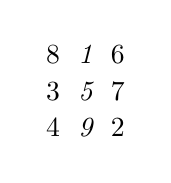
\begin{tikzpicture}
  [matrix of nodes/.style={
     execute at begin cell=\node\bgroup,
     execute at end cell=\egroup;%
   }]
  \matrix [matrix of nodes]
  {
    8 & 1 & 6 \\
    3 & 5 & 7 \\
    4 & 9 & 2 \\
  };
\end{tikzpicture}
\end{codeexample}
%
\begin{codeexample}[]
\begin{tikzpicture}
  [matrix of nodes/.style={
     execute at begin cell=\node\bgroup,
     execute at end cell=\egroup;,%
     execute at empty cell=\node{--};%
   }]
  \matrix [matrix of nodes]
  {
    8 & 1 &   \\
    3 &   & 7 \\
      &   & 2 \\
  };
\end{tikzpicture}
\end{codeexample}

The |matrix| library defines a number of styles that make use of the above
options.

|matrix| 库定义了许多使用上述选项的样式。


\subsection{Anchoring a Matrix\\矩阵的定位}

Since matrices are nodes, they can be anchored in the usual fashion using the
|anchor| option. However, there are two ways to influence this placement
further. First, the following option is often useful:

由于矩阵是节点,所以可以使用 |anchor| 选项按照通常的方式对其进行定位。然而,还有两种方法可以进一步影响此定位。首先,以下选项通常很有用:

\begin{key}{/tikz/matrix anchor=\meta{anchor}}
    This option has the same effect as |anchor|, but the option applies only to
    the matrix itself, not to the cells inside. If you just say |anchor=north|
    as an option to the matrix node, all nodes inside matrix will also have
    this anchor, unless it is explicitly set differently for each node. By
    comparison, |matrix anchor| sets the anchor for the matrix, but for the
    nodes inside the value of |anchor| remain unchanged.
    
    此选项与 |anchor| 具有相同的效果,但该选项仅适用于矩阵本身,不适用于其中的单元格。如果您只是将 |anchor=north| 作为矩阵节点的选项,除非为每个节点明确设置了不同的锚点,否则矩阵内的所有节点也都将具有此锚点。相比之下,|matrix anchor| 设置了矩阵的锚点,但对于节点内的值,|anchor| 的值保持不变。


\begin{codeexample}[]
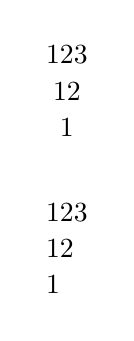
\begin{tikzpicture}
  \matrix [matrix anchor=west] at (0,0)
  {
    \node {123}; \\ % still center anchor
    \node {12}; \\
    \node {1}; \\
  };
  \matrix [anchor=west] at (0,-2)
  {
    \node {123}; \\ % inherited west anchor
    \node {12}; \\
    \node {1}; \\
  };
\end{tikzpicture}
\end{codeexample}
    %
\end{key}

The second way to anchor a matrix is to use \emph{an anchor of a node inside
the matrix}. For this, the |anchor| option has a special effect when given as
an argument to a matrix:

定位矩阵的第二种方法是使用\emph{矩阵内某个节点的锚点}。为此,当作为矩阵的参数给出时,|anchor| 选项具有特殊效果:

\begin{key}{/tikz/anchor=\meta{anchor or node.anchor}}
    Normally, the argument of this option refers to anchor of the matrix node,
    which is the node that includes all of the stuff of the matrix. However,
    you can also provide an argument of the form \meta{node}|.|\meta{anchor}
    where \meta{node} must be node defined inside the matrix and \meta{anchor}
    is an anchor of this node. In this case, the whole matrix is shifted around
    in such a way that this particular anchor of this particular node lies at
    the |at| position of the matrix. The same is true for |matrix anchor|.
    
    通常,此选项的参数是矩阵节点的锚点,该节点包含矩阵的所有内容。但是,您还可以提供形式为 \meta{node}|.|\meta{anchor} 的参数,其中 \meta{node} 必须是在矩阵内定义的节点,而 \meta{anchor} 是该节点的一个锚点。在这种情况下,整个矩阵将以这个特定节点的这个特定锚点位于矩阵的 |at| 位置的方式进行移动。|matrix anchor| 的情况与此类似。


\begin{codeexample}[]
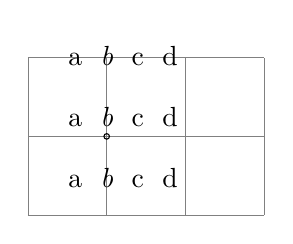
\begin{tikzpicture}
  \draw[help lines] (0,0) grid (3,2);
  \matrix[matrix anchor=inner node.south,anchor=base,row sep=3mm] at (1,1)
  {
    \node {a}; & \node             {b}; & \node {c}; & \node {d}; \\
    \node {a}; & \node(inner node) {b}; & \node {c}; & \node {d}; \\
    \node {a}; & \node             {b}; & \node {c}; & \node {d}; \\
  };
  \draw (inner node.south) circle (1pt);
\end{tikzpicture}
\end{codeexample}
    %
\end{key}


\subsection{Considerations Concerning Active Characters\\关于活动字符的考虑}

Even though \tikzname\ seems to use |&| to separate cells, \pgfname\ actually
uses a different command to separate cells, namely the command
|\pgfmatrixnextcell| and using a normal |&| character will normally fail. What
happens is that, \tikzname\ makes |&| an active character and then defines this
character to be equal to |\pgfmatrixnextcell|. In most situations this will
work nicely, but sometimes |&| cannot be made active; for instance because the
matrix is used in an argument of some macro or the matrix contains nodes that
contain normal |{tabular}| environments. In this case you can use the following
option to avoid having to type |\pgfmatrixnextcell| each time:

尽管 \tikzname\ 似乎使用 |&| 来分隔单元格,但实际上 \pgfname\ 使用了不同的命令来分隔单元格,即命令 |\pgfmatrixnextcell|,使用普通的 |&| 字符通常会失败。实际上,\tikzname\ 将 |&| 设置为活动字符,然后将此字符定义为等于 |\pgfmatrixnextcell|。在大多数情况下,这样做效果很好,但有时候 |&| 无法设置为活动字符;例如,因为矩阵在某些宏的参数中使用,或者矩阵包含包含普通的 |{tabular}| 环境的节点。在这种情况下,可以使用以下选项,以避免每次都键入 |\pgfmatrixnextcell|:

\begin{key}{/tikz/ampersand replacement=\meta{macro name or empty}}
    If a macro name is provided, this macro will be defined to be equal to
    |\pgfmatrixnextcell| inside matrices and |&| will not be made active. For
    instance, you could say |ampersand replacement=\&| and then use |\&| to
    separate columns as in the following example:
    
    如果提供了一个宏名,该宏将在矩阵内定义为等于 |\pgfmatrixnextcell|,而 |&| 将不会被设置为活动字符。例如,可以使用 |ampersand replacement=&|,然后在以下示例中使用 |&| 来分隔列:


\begin{codeexample}[]
\tikz
  \matrix [ampersand replacement=\&]
  {
    \draw (0,0)   circle (4mm); \& \node[rotate=10] {Hello};        \\
    \draw (0.2,0) circle (2mm); \& \fill[red]   (0,0) circle (3mm); \\
  };
\end{codeexample}
    %
\end{key}


\subsection{Examples\\示例}

The following examples are adapted from code by Mark Wibrow. The first two
redraw pictures from Timothy van Zandt's PStricks documentation:

以下示例改编自 Mark Wibrow 的代码。前两个示例重新绘制了 Timothy van Zandt 的 PStricks 文档中的图片:


{\catcode`\|=12
\begin{codeexample}[preamble={\usetikzlibrary{matrix}}]
\begin{tikzpicture}
  \matrix [matrix of math nodes,row sep=1cm]
  {
    |(U)| U &[2mm]                       &[8mm]    \\
            &      |(XZY)| X \times_Z Y  &      |(X)| X \\
            &      |(Y)|   Y             &      |(Z)| Z \\
  };
  \begin{scope}[every node/.style={midway,auto,font=\scriptsize}]
    \draw [double, dashed] (U)   -- node {$x$} (X);
    \draw                  (X)   -- node {$p$} (X -| XZY.east)
                           (X)   -- node {$f$} (Z)
                                 -- node {$g$} (Y)
                                 -- node {$q$} (XZY)
                                 -- node {$y$} (U);
   \end{scope}
\end{tikzpicture}
\end{codeexample}

\begin{codeexample}[
    preamble={\usetikzlibrary{matrix}},
    pre={\definecolor{graphicbackground}{rgb}{0.96,0.96,0.8}},
]
\begin{tikzpicture}[>=stealth,->,shorten >=2pt,looseness=.5,auto]
  \matrix [matrix of math nodes,
           column sep={2cm,between origins},
           row sep={3cm,between origins},
           nodes={circle, draw, minimum size=7.5mm}]
  {
            & |(A)| A &         \\
    |(B)| B & |(E)| E & |(C)| C \\
            & |(D)| D           \\
  };
  \begin{scope}[every node/.style={font=\small\itshape}]
    \draw (A) to [bend left] node [midway]   {g} (B);
    \draw (B) to [bend left] node [midway]   {f} (A);
    \draw (D) --             node [midway]   {c} (B);
    \draw (E) --             node [midway]   {b} (B);
    \draw (E) --             node [near end] {a} (C);
    \draw [-,line width=8pt,draw=graphicbackground]
          (D) to [bend right, looseness=1] (A);
    \draw (D) to [bend right, looseness=1]
            node [near start] {b} node [near end] {e} (A);
  \end{scope}
\end{tikzpicture}
\end{codeexample}

\begin{codeexample}[preamble={\usetikzlibrary{matrix}}]
\begin{tikzpicture}
  \matrix (network)
    [matrix of nodes,%
     nodes in empty cells,
     nodes={outer sep=0pt,circle,minimum size=4pt,draw},
     column sep={1cm,between origins},
     row sep={1cm,between origins}]
  {
                  &                &                 & \\
                  &                &                 & \\
    |[draw=none]| & |[xshift=1mm]| & |[xshift=-1mm]|   \\
  };
  \foreach \a in {1,...,4}{
    \draw (network-3-2) -- (network-2-\a);
    \draw (network-3-3) -- (network-2-\a);
    \draw [-stealth] ([yshift=5mm]network-1-\a.north) -- (network-1-\a);
    \foreach \b in {1,...,4}
      \draw (network-1-\a) -- (network-2-\b);
  }
  \draw [stealth-] ([yshift=-5mm]network-3-2.south) -- (network-3-2);
  \draw [stealth-] ([yshift=-5mm]network-3-3.south) -- (network-3-3);
\end{tikzpicture}
\end{codeexample}

The following example is adapted from code written by Kjell Magne Fauske, which
is based on the following paper: K.~Bossley, M.~Brown, and C.~Harris,
Neurofuzzy identification of an autonomous underwater vehicle,
\emph{International Journal of Systems Science}, 1999, 30, 901--913.

以下示例改编自 Kjell Magne Fauske 的代码,该代码基于以下论文:K.~Bossley、M.~Brown 和 C.~Harris,Neurofuzzy identification of an autonomous underwater vehicle,\emph{International Journal of Systems Science},1999,30,901--913。


\begin{codeexample}[preamble={\usetikzlibrary{arrows,shapes.geometric}}]
\begin{tikzpicture}
  [auto,
   decision/.style={diamond, draw=blue, thick, fill=blue!20,
                    text width=4.5em,align=flush center,
                    inner sep=1pt},
   block/.style   ={rectangle, draw=blue, thick, fill=blue!20,
                    text width=5em,align=center, rounded corners,
                    minimum height=4em},
   line/.style    ={draw, thick, -latex',shorten >=2pt},
   cloud/.style   ={draw=red, thick, ellipse,fill=red!20,
                    minimum height=2em}]

  \matrix [column sep=5mm,row sep=7mm]
  {
    % row 1
      \node [cloud] (expert)   {expert}; &
      \node [block] (init)     {initialize model}; &
      \node [cloud] (system)   {system}; \\
    % row 2
      & \node [block] (identify) {identify candidate model}; & \\
    % row 3
      \node [block] (update)   {update model};  &
      \node [block] (evaluate) {evaluate candidate models}; & \\
    % row 4
      & \node [decision] (decide) {is best candidate}; & \\
    % row 5
      & \node [block] (stop)      {stop}; & \\
  };
  \begin{scope}[every path/.style=line]
    \path          (init)     -- (identify);
    \path          (identify) -- (evaluate);
    \path          (evaluate) -- (decide);
    \path          (update)   |- (identify);
    \path          (decide)   -| node [near start] {yes} (update);
    \path          (decide)   -- node [midway] {no} (stop);
    \path [dashed] (expert)   -- (init);
    \path [dashed] (system)   -- (init);
    \path [dashed] (system)   |- (evaluate);
  \end{scope}
\end{tikzpicture}
\end{codeexample}
}


%%% Local Variables:
%%% mode: latex
%%% TeX-master: "pgfmanual"
%%% End:
